\documentclass[11pt]{article}

\usepackage[margin=1in]{geometry}
\usepackage{times}
\usepackage{amsmath,amssymb}
\usepackage{graphicx}
\usepackage{booktabs}
\usepackage{hyperref}
\usepackage{url}
\usepackage{enumitem}

\title{
StealthRL: Ensemble-Guided Text Transformation for\\
Multi-Detector Transfer and Fair Detection Robustness
}

\author{
Suraj Ranganath, Sibo Zhu, Nishchay Mahor\\
\small Halicioğlu Data Science Institute, University of California San Diego\\
\small \texttt{\{suranganath, siz030, nmahor\}@ucsd.edu}
}

\date{December 8, 2025}

\begin{document}

\maketitle

\begin{abstract}
AI-generated text detectors are increasingly deployed in academic integrity workflows, content moderation, and misinformation pipelines. However, current detectors are brittle to paraphrasing attacks and exhibit systematic bias against English-as-a-Second-Language (ESL) writers. Prior adversarial work such as AuthorMist trains separate reinforcement learning (RL) policies per detector and treats fairness as a purely post-hoc analysis problem. 

We present StealthRL, a reinforcement learning framework that fine-tunes a single paraphraser against an ensemble of AI-text detectors while explicitly optimizing for semantic fidelity, fluency, and ESL fairness. StealthRL uses Group Relative Policy Optimization (GRPO) together with low-rank adaptation (LoRA) on Qwen3-4B-Instruct to learn detector-agnostic transformation strategies. Our reward function combines an ensemble-based detection score, embedding-based semantic similarity, language-model perplexity, and a novel ESL fairness penalty that downweights policies that disproportionately increase detector scores on ESL text.

As a proof-of-concept, we train StealthRL for 50 GRPO steps on 800 examples using Fast-DetectGPT as the sole detector. This ultra-fast run improves detector evasion by roughly 22\% (reduction in detection probability from 58.7\% to 45.8\% at the best checkpoint) while maintaining an average semantic similarity of 98.6\% and preventing model collapse (parse success 85.9\% $\rightarrow$ 99.2\%, KL divergence $<0.4$). We identify nine Pareto-optimal checkpoints that trade off stealth, semantic preservation, and naturalness. We also design a full production configuration---20k examples, three-detector ensemble (Fast-DetectGPT, Ghostbuster, Binoculars), 40\% ESL / 60\% native split---with a projected attack success rate (ASR) of 60--70\% and a targeted 50--80\% reduction in ESL false-positive gaps. 

Our contribution is both algorithmic and engineering: we (i) apply GRPO to adversarial NLP with multi-objective and fairness-aware rewards, (ii) build a multi-detector, fairness-aware training harness that the research community can use to train paraphrasers against detector ensembles, and (iii) provide a reproducible, open-source codebase and configuration suite that can be reused for red-teaming and for studying the detector--evader arms race.

Code and configurations are available at \url{https://github.com/suraj-ranganath/StealthRL} (currently private as we plan to continue work on this project; access can be granted for evaluation or collaboration purposes upon request to \texttt{suranganath@ucsd.edu}).
\end{abstract}

\section{Introduction}

Large language models (LLMs) are now widely used to assist with writing in academic, professional, and creative contexts. In parallel, AI-generated text detectors are deployed to enforce academic integrity, detect synthetic news, and support content moderation. Despite their growing use, these detectors suffer from two fundamental problems:

\begin{itemize}[leftmargin=*]
    \item \textbf{Brittleness to paraphrasing:} Zero-shot methods such as DetectGPT and its efficient variants achieve high AUROC on unmodified LLM text, but their performance drops sharply after simple paraphrasing. Prior work has shown AUROC degradation from $\sim$95\% to $\sim$60\% under paraphrase-based attacks.
    \item \textbf{Bias against ESL writers:} Recent analyses have found that TOEFL essays and other ESL corpora are flagged as AI-generated at 2--3$\times$ the rate of comparable native writing, raising serious fairness concerns in educational and professional environments.
\end{itemize}

Existing adversarial work such as AuthorMist and DIPPER focuses on maximizing detector evasion, typically by training one RL policy per detector or by using purely prompt-based paraphrasing. These approaches do not systematically study \emph{multi-detector generalization}, nor do they integrate fairness constraints into the training objective.

\subsection{Problem Statement}

We study the problem of learning a \emph{single} paraphrase policy that:

\begin{enumerate}[leftmargin=*]
    \item Achieves strong attack success rates (ASR) against multiple detector families (curvature-based, classifier-based, and paired-LM),
    \item Preserves the original semantic content and maintains human-like fluency, and
    \item Reduces detector bias against ESL writers by explicitly penalizing unfair detection behaviour during training.
\end{enumerate}

\subsection{Research Questions}

We organize our investigation around three research questions:

\begin{description}[leftmargin=*]
    \item[RQ1: Multi-detector generalization.] Does training on a 2-detector ensemble (e.g., Fast-DetectGPT + Ghostbuster) transfer to a held-out detector family (e.g., Binoculars)? We measure the \emph{transfer ratio} ASR$_{\text{held-out}}$/ASR$_{\text{in-ensemble}}$ and target values above 0.7.
    \item[RQ2: Reward component necessity.] Which reward components (detection, semantics, fluency, fairness) are necessary to obtain good trade-offs between stealth and quality? We design five ablation studies to test the contribution of each term.
    \item[RQ3: Fairness in adversarial RL.] Can an explicit ESL penalty in the RL reward reduce the false-positive rate (FPR) gap between ESL and native writers by 50--80\%, targeting an absolute gap below 0.07?
\end{description}

\subsection{Contributions}

Our main contributions are:

\begin{itemize}[leftmargin=*]
    \item \textbf{StealthRL framework.} We introduce a GRPO-based RL framework that fine-tunes Qwen3-4B-Instruct with LoRA adapters to paraphrase AI-generated text while optimizing a multi-objective reward over detection, semantic similarity, naturalness, and fairness.
    \item \textbf{Fairness-aware adversarial training.} We propose, to our knowledge, the first ESL-specific fairness penalty integrated directly into the adversarial training loop, rather than applied post-hoc.
    \item \textbf{Multi-detector, detector-agnostic training.} We design an ensemble of locally-hosted, open-source detectors (Fast-DetectGPT, Ghostbuster, Binoculars) and study cross-family generalization and held-out detector transfer within this framework.
    \item \textbf{Evaluation and tooling.} We implement StealthBench, a multi-detector evaluation harness with low-FPR and fairness metrics, as well as a full pipeline for training, evaluation, and visualization on the Tinker platform.
\end{itemize}

\section{Related Work}

\subsection{AI-Text Detection}

Detection methods broadly fall into three families:

\paragraph{Curvature-based detectors.}
DetectGPT~\cite{mitchell2023detectgpt} identifies AI-generated text by comparing log-probabilities of candidate continuations under a base language model at sampled perturbations; AI text tends to lie in high-probability, low-curvature regions. Fast-DetectGPT~\cite{bao2024fastdetect} improves efficiency by using conditional probability curvature, making it more suitable for large-scale evaluation and RL feedback.

\paragraph{Classifier-based detectors.}
Classifier-based approaches train discriminative models (often transformer-based) to label text as human or AI. Ghostbuster~\cite{verma2024ghostbuster} uses an ensemble of over a hundred hand-engineered features and a RoBERTa classifier to detect LLM-authored writing. Such models are sensitive to the distribution of their training data and may struggle with out-of-domain text.

\paragraph{Paired-LM detectors.}
Binoculars~\cite{hans2024binoculars} compares probabilities from a base LM and an instruction-tuned variant; human text tends to score higher under the latter. This architecture requires no explicit classifier training and can generalize across domains, making it an attractive held-out detector.

\subsection{Evasion and Adversarial Paraphrasing}

Paraphrase-based attacks aim to transform AI-generated text into a form that evades detectors while preserving meaning. DIPPER~\cite{krishna2023dipper} demonstrates that controlled paraphrasing can dramatically lower the performance of common detectors, while SICO~\cite{lu2024sico} uses in-context optimization and token substitution attacks without fine-tuning.

AuthorMist~\cite{david2025authormist} introduces reinforcement learning with detector feedback and reports 60--80\% ASR per detector, but trains a separate policy for each detector and does not study multi-detector transfer or fairness effects.

\subsection{Fairness and Bias in AI-Text Detection}

Liang et al.~\cite{liang2023bias} show that GPT detectors are biased against non-native English writing: TOEFL essays are flagged as AI-generated 2--3$\times$ more often than native essays. They release the ChatGPT-Detector-Bias dataset and call for fair detection methods. To date, adversarial paraphrasing work has largely ignored fairness as a training objective; fairness analyses are typically performed post-hoc. StealthRL is designed to close this gap by explicitly including an ESL-specific penalty in the reward.

\section{Method}

\subsection{Problem Formulation}

We consider a base LLM that generates an AI-authored text $x$ given a prompt. Our goal is to learn a paraphrase policy $\pi_\theta(y \mid x)$ that outputs a paraphrase $y$ such that:

\begin{itemize}[leftmargin=*]
    \item Multiple detectors $D_1, \dots, D_m$ assign low probability of AI authorship to $y$,
    \item $y$ preserves the semantics of $x$ and remains fluent, and
    \item The gap in false-positive rates between ESL and native text is reduced.
\end{itemize}

We treat $\pi_\theta$ as a parameter-efficient LoRA adaptation of Qwen3-4B-Instruct and train it via GRPO with a scalar reward $R(x,y)$ that aggregates multiple objectives.

\subsection{Model and Architecture}

Our policy model is Qwen/Qwen3-4B-Instruct-2507 with LoRA adapters on all linear layers in the attention and MLP blocks. Only the LoRA parameters are trained:

\begin{equation}
W_{\text{eff}} = W_{\text{base}} + \frac{\alpha}{r} B A,
\end{equation}

where $A \in \mathbb{R}^{d_{\text{in}} \times r}$ and $B \in \mathbb{R}^{r \times d_{\text{out}}}$ are low-rank matrices, $r$ is the LoRA rank, and $\alpha$ is a scaling factor. We use ranks $r=16$ (ultra-fast proof-of-concept) and $r=32$ (planned production), with matching $\alpha$.

The complete experimental pipeline including evaluation, transfer learning, ablations, and baseline comparisons is shown in Figure~\ref{fig:pipeline-overview}. The GRPO training loop at the core of this pipeline is illustrated in detail in Figure~\ref{fig:pipeline}. At each training step, the LoRA-augmented policy generates $K$ paraphrases per prompt, a composite reward is computed based on detectors, semantic similarity, perplexity, and fairness, and GRPO updates the LoRA parameters using group-relative advantages with KL regularization.

\begin{figure}[htbp]
    \centering
    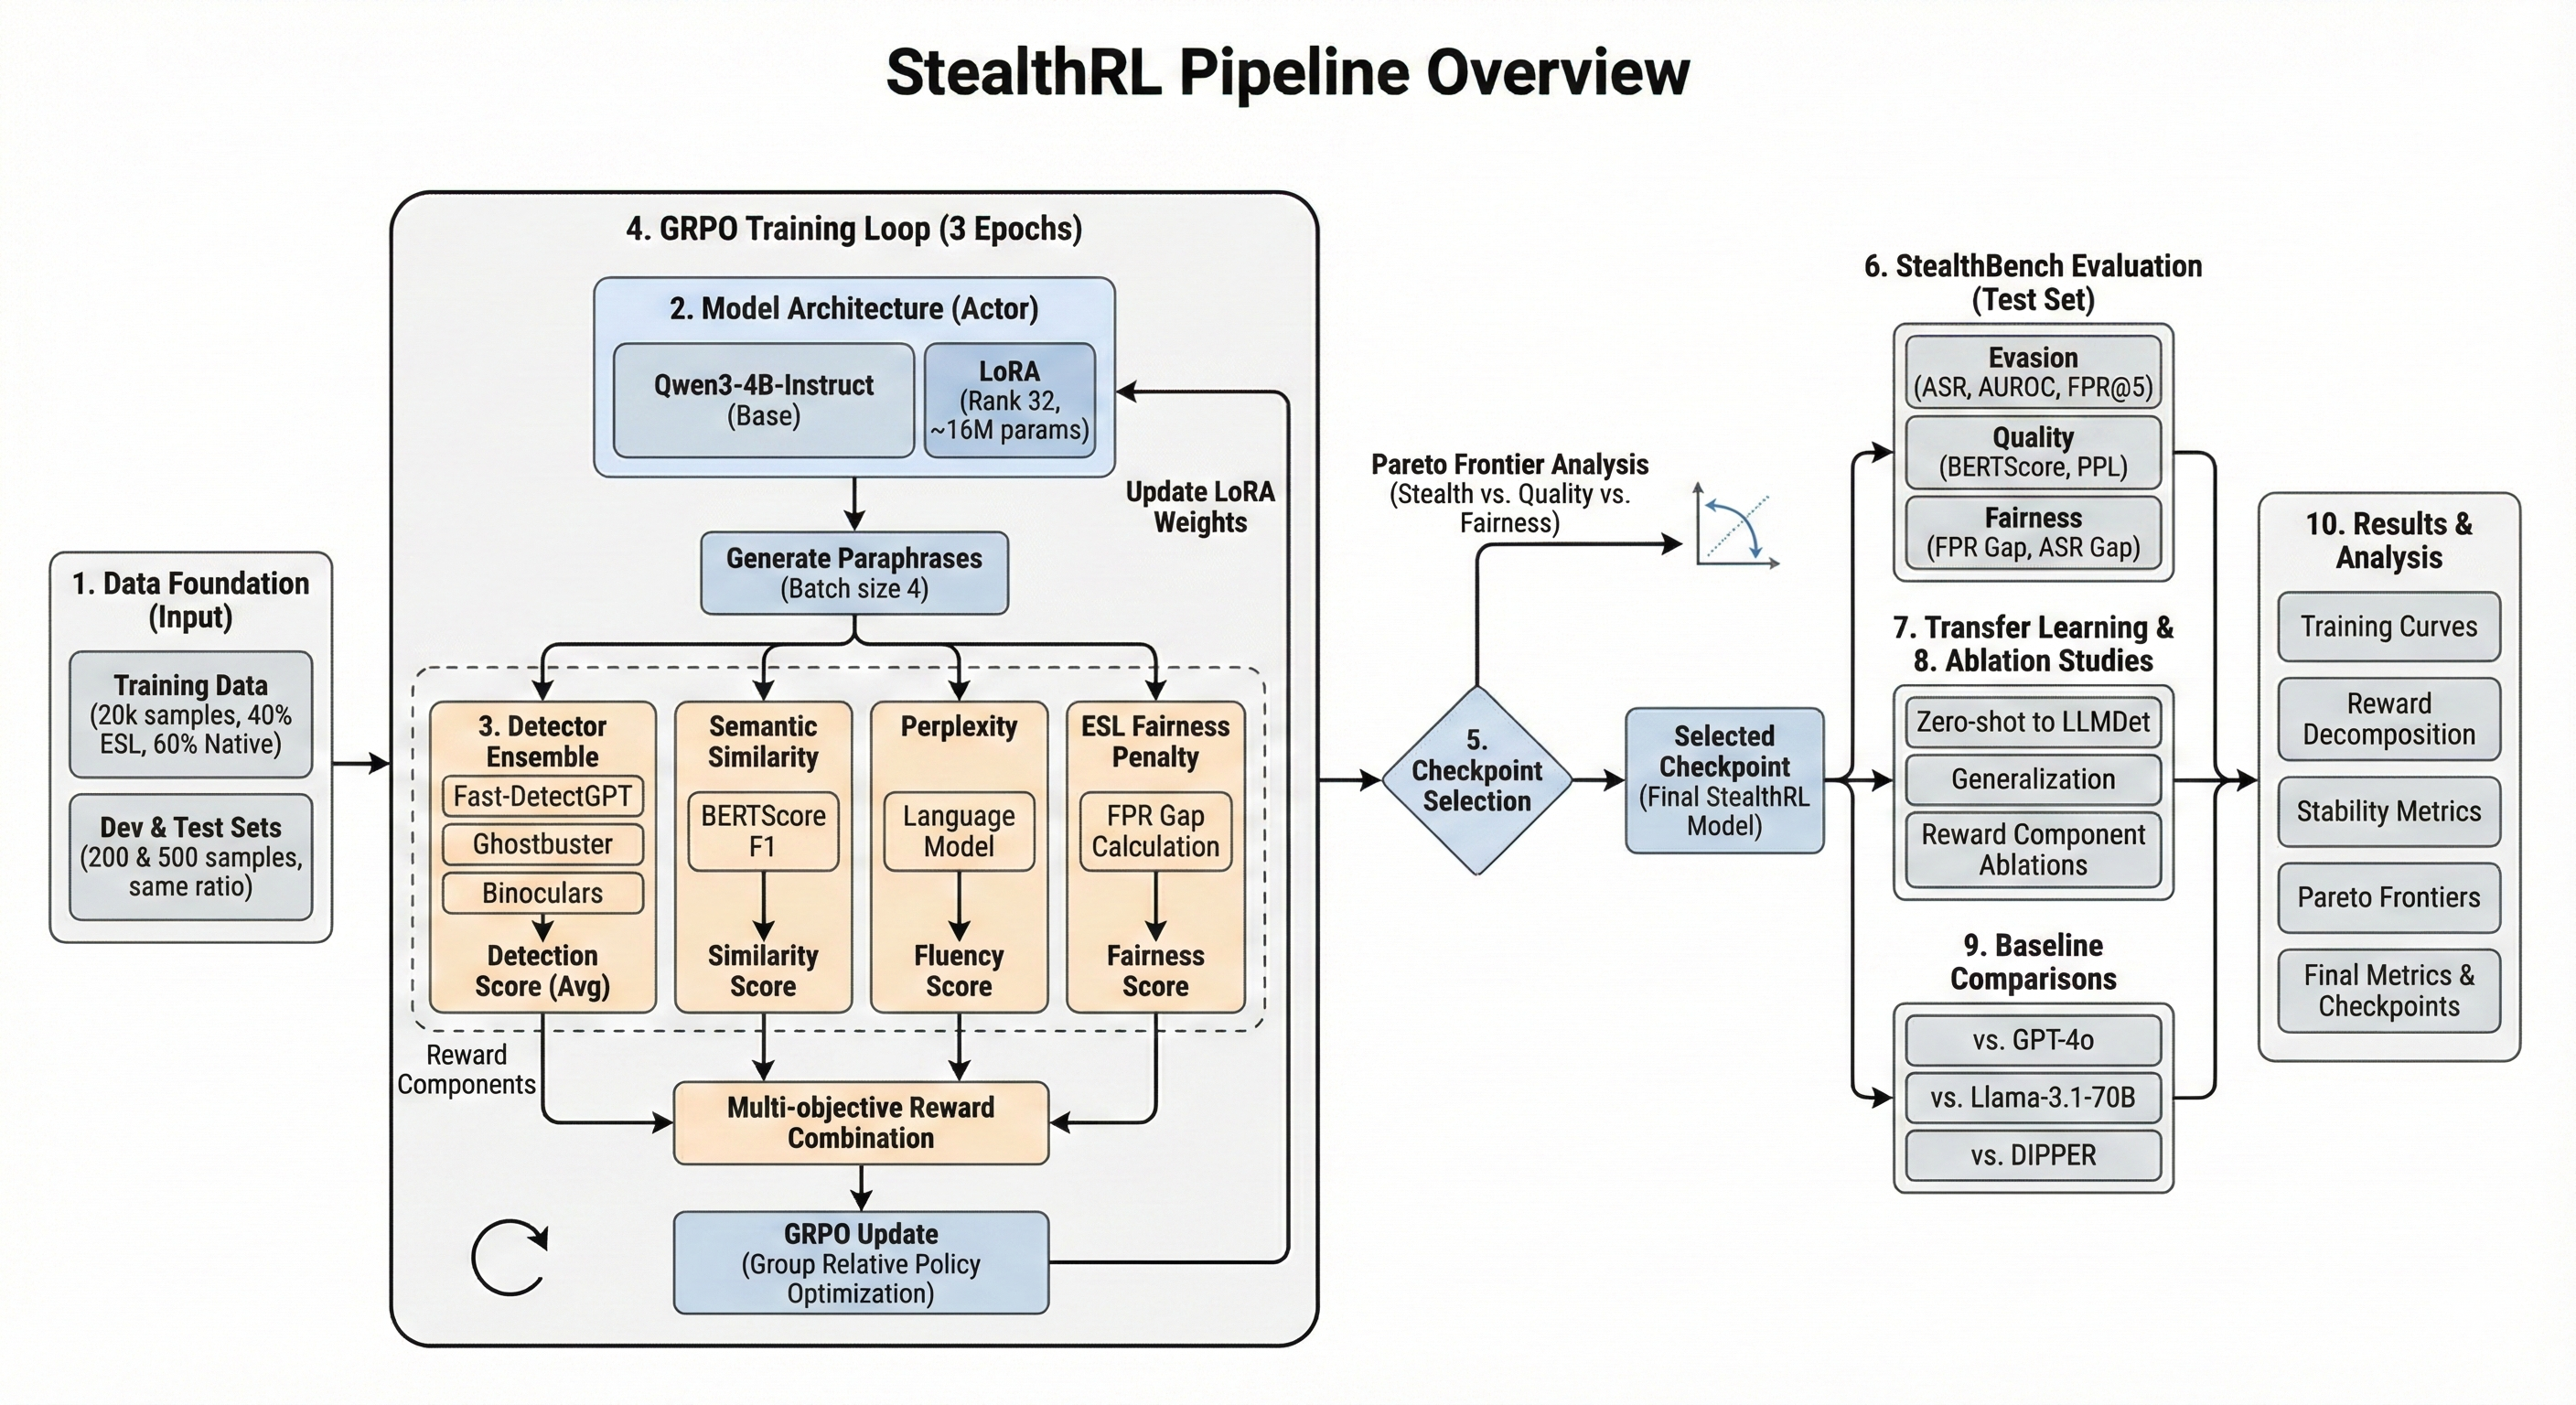
\includegraphics[width=\textwidth]{StealthRL_Methodology.png}
    \caption{StealthRL complete experimental pipeline overview. The full-scale experiment begins with data foundation (20k training samples, 40\% ESL / 60\% native), proceeds through GRPO training with multi-detector ensemble and multi-objective rewards over 3 epochs, performs Pareto frontier analysis to select optimal checkpoints balancing stealth, quality, and fairness, evaluates on StealthBench test set, conducts transfer learning to unseen detectors (LLMDet), performs ablation studies on reward components, compares against baselines (GPT-4o, Llama-3.1-70B, DIPPER), and generates comprehensive results analysis including training curves, reward decomposition, stability metrics, Pareto frontiers, and final performance metrics.}
    \label{fig:pipeline-overview}
\end{figure}

\begin{figure}[htbp]
    \centering
    \includegraphics[width=\textwidth]{../outputs/tinker_ultrafast/run_20251207_212110/visualizations/stealthrl_pipeline.png}
    \caption{StealthRL training pipeline. The system takes human reference text with ESL/native labels as input, uses a LoRA-adapted Qwen-3B policy to generate $K$ paraphrased candidates via on-policy sampling, computes a composite reward from four components (detector ensemble, semantic fidelity, fluency, and fairness penalty), and updates the LoRA adapter weights via GRPO in a closed loop. The detector cache (SQLite) enables efficient reward computation during training.}
    \label{fig:pipeline}
\end{figure}

\subsection{Composite Reward Function}

We define the overall reward as
\begin{equation}
R_{\text{total}} = \alpha R_{\text{det}} + \beta R_{\text{sem}} + \gamma R_{\text{ppl}} - \delta R_{\text{fair}},
\end{equation}
with default weights $\alpha = 1.0$, $\beta = 1.0$, $\gamma = 0.5$, and $\delta = 0.2$.

\paragraph{Detector reward $R_{\text{det}}$.}
Let $p_i(x)$ be the probability that detector $D_i$ assigns to ``AI'' for text $x$, and $w_i$ be ensemble weights. The ensemble detection probability is
\[
p_{\text{ens}}(y) = \frac{\sum_i w_i \, p_i(y)}{\sum_i w_i}.
\]
We define a raw detector reward $r_{\text{det}} = 1 - p_{\text{ens}}(y)$ (higher is better) and apply running z-score normalization followed by clipping:
\[
R_{\text{det}} = \mathrm{clip}\left( \frac{r_{\text{det}} - \mu_t}{\sigma_t + \epsilon}, -3, 3 \right).
\]

\paragraph{Semantic reward $R_{\text{sem}}$.}
We embed $x$ and $y$ with an E5 encoder (e.g., \texttt{intfloat/e5-small-v2} for the ultra-fast run) and compute cosine similarity $s = \cos(e(x), e(y))$. We use a thresholded reward:
\[
R_{\text{sem}} =
\begin{cases}
s, & s \ge 0.85,\\
s - 0.5, & s < 0.85,
\end{cases}
\]
which heavily penalizes significant semantic drift.

\paragraph{Fluency reward $R_{\text{ppl}}$.}
We approximate naturalness via perplexity $\text{ppl}(y)$ under a small language model (GPT-2). We specify a target range $[\text{ppl}_{\min}, \text{ppl}_{\max}]$ and a target value $\text{ppl}_\star$ representing typical human text:
\[
R_{\text{ppl}} =
\begin{cases}
1 - \dfrac{|\text{ppl}(y) - \text{ppl}_\star|}{\text{ppl}_{\max} - \text{ppl}_{\min}}, & \text{ppl}_{\min} \le \text{ppl}(y) \le \text{ppl}_{\max},\\[0.5em]
-1, & \text{otherwise}.
\end{cases}
\]

\paragraph{Fairness penalty $R_{\text{fair}}$.}
For samples labeled as ESL, we penalize high detector scores:
\[
R_{\text{fair}} =
\begin{cases}
p_{\text{ens}}(y), & \text{if sample is ESL},\\
0, & \text{otherwise}.
\end{cases}
\]
This term encourages the model to reduce detector confidence specifically on ESL text, without directly altering rewards for native text. The penalty is multiplied by $\delta$ in $R_{\text{total}}$.

\subsection{Group Relative Policy Optimization}

We adopt Group Relative Policy Optimization (GRPO)~\cite{shao2024grpo}, a variant of PPO that removes the need for a learned value function. For each prompt $x$ in a batch, we generate a group of $K$ rollouts $\{y_1, \dots, y_K\}$, compute rewards $\{R_k\}$, and normalize within-group:

\begin{align}
\mu_g &= \frac{1}{K} \sum_{k=1}^K R_k,\quad
\sigma_g = \sqrt{\frac{1}{K} \sum_{k=1}^K (R_k - \mu_g)^2 + \epsilon},\\
A_k &= \mathrm{clip}\left( \frac{R_k - \mu_g}{\sigma_g}, -c, c \right),
\end{align}
where $c$ is an advantage clip (e.g., $c=5$ in the ultra-fast run).

Let $\pi_\theta$ be the current policy and $\pi_{\text{ref}}$ a frozen reference policy (the base model or an early checkpoint). The GRPO loss is
\begin{equation}
\mathcal{L}_{\text{GRPO}}(\theta) = -\mathbb{E}\left[A_k \log \frac{\pi_\theta(y_k \mid x)}{\pi_{\text{ref}}(y_k \mid x)}\right] + \beta_{\text{KL}} \, \mathrm{KL}\big(\pi_\theta(\cdot \mid x)\,\|\,\pi_{\text{ref}}(\cdot \mid x)\big),
\end{equation}
with $\beta_{\text{KL}}$ tuned either adaptively (ultra-fast run) or fixed (planned full run). Only the LoRA parameters are updated.

We found that grouping with $K=8$ rollouts per prompt is critical: smaller $K$ leads to many groups with nearly constant rewards, collapsing the advantage signal.

\subsection{Training Stability Mechanisms}

To prevent model collapse and excessive drift:

\begin{itemize}[leftmargin=*]
    \item We monitor KL divergence and use an adaptive penalty to keep it below a target (4.0 in the ultra-fast run).
    \item We clip both rewards and advantages to mitigate the influence of outliers.
    \item We use cosine learning-rate schedules with a 10\% warmup.
    \item We detect ``all-negative'' or low-variance groups and downweight or adjust them to maintain useful gradients.
    \item We track a simple parse-success metric (e.g., fraction of outputs meeting format constraints) as a proxy for catastrophic failure.
\end{itemize}

These mechanisms are validated in Section~\ref{sec:results-ultrafast}, with detailed stability metrics shown in Figure~\ref{fig:stability-metrics}.

\section{Implementation and Infrastructure}

\subsection{Codebase Overview}

The StealthRL codebase is organized into modular components:

\begin{itemize}[leftmargin=*]
    \item \texttt{detectors/}: wrappers for Fast-DetectGPT, Ghostbuster, and Binoculars, with thread-safe singleton loading and SQLite-based caching to avoid repeated computation.
    \item \texttt{rewards/}: detector, semantic, quality, and fairness reward components plus a composite aggregator.
    \item \texttt{tinker/}: integration with the Tinker platform, including GRPO environment, dataset handling, training, inference, and evaluation.
    \item \texttt{data/}: ESL/native corpus loaders for TOEFL-like and native corpora with a unified schema and stratified sampling utilities.
    \item \texttt{evaluation/}: the StealthBench harness for ASR, AUROC, low-FPR, semantic, and fairness metrics.
    \item \texttt{scripts/}: data preparation, training, transfer evaluation, ESL fairness analysis, and visualization.
\end{itemize}

In total, the project comprises roughly 6k lines of Python code spanning core training, evaluation, and tooling.

\subsection{Detector Ensemble Implementation}

All detectors are locally hosted:

\begin{itemize}[leftmargin=*]
    \item \textbf{Fast-DetectGPT:} a curvature-based detector using conditional probability curvature, selected as the fastest reward component.
    \item \textbf{Ghostbuster:} a RoBERTa-based classifier with a rich feature set.
    \item \textbf{Binoculars:} a paired-LM detector comparing base and instruction-tuned probabilities.
\end{itemize}

To avoid race conditions and meta-tensor errors, we wrap model loading in a thread-safe cache and cache per-text detector outputs in SQLite keyed by a hash of the text. After warmup, cache hit rates exceed 90\%, yielding order-of-magnitude speedups in RL training.

\subsection{Tinker Platform and Compute}

We use the Tinker platform (Thinking Machines Lab) for remote GRPO training on Qwen3-4B-Instruct:

\begin{itemize}[leftmargin=*]
    \item \textbf{Ultra-fast run:} 800 training examples, 1 epoch, 50 GRPO steps on a single A100 40GB GPU, taking roughly 3.5 hours.
    \item \textbf{Planned full run:} 20k+ training examples, 3 epochs, three-detector ensemble, expected 6--8 hours on the same hardware.
\end{itemize}

The implementation follows best practices from the Tinker LLM docs and agents cookbook, as well as public guidance on LoRA with RL and GRPO hyperparameter tuning.

\section{Experimental Setup}

\subsection{Datasets}

We construct an ESL/native corpus by combining:

\begin{itemize}[leftmargin=*]
    \item ESL sources such as the ELLIPSE (Kaggle Feedback Prize) and ICNALE corpora, providing essays from non-native English learners across multiple CEFR levels and countries.
    \item Native sources such as subsets of DetectRL, covering academic abstracts, news, and creative writing authored by native speakers.
\end{itemize}

For the planned full run, we curate a split with 40\% ESL and 60\% native texts in both train and test to support fairness analysis. For the ultra-fast proof-of-concept, we sample 800 training and 150 test examples without enforcing balance, which limits fairness conclusions but is adequate to validate training stability.

Each example includes: AI-generated text $x$, an optional human reference, a domain label (academic, news, creative), an ESL flag, and the corpus source.

\subsection{Research Questions and Experiments}

We design experiments to address our research questions:

\paragraph{Core training and ultra-fast validation.}
We train StealthRL on 800 examples using only Fast-DetectGPT as the detector to test whether GRPO + LoRA can be stabilized with a multi-objective reward. This is the experiment reported in detail in Section~\ref{sec:results-ultrafast}.

\paragraph{Full ensemble and transfer (RQ1).}
We plan a full run on 20k examples where the training ensemble includes Fast-DetectGPT, Ghostbuster, and Binoculars. A separate transfer configuration trains on Fast-DetectGPT + Ghostbuster and evaluates ASR on held-out Binoculars to measure cross-family generalization.

\paragraph{Reward ablations (RQ2).}
We define five ablation settings: detector-only, no fairness, no quality, no semantic constraint, and single-detector training. Each is trained under similar budgets, and we compare ASR, semantic similarity, perplexity, and ESL fairness to the full model.

\paragraph{Fairness analysis (RQ3).}
Using the ESL-balanced test set, we compute FPR(ESL) $-$ FPR(native) for each detector and model variant (base, SFT, StealthRL with/without fairness term), along with AUROC gaps and semantic similarity stratified by ESL vs native.

\subsection{Metrics}

We evaluate along four axes:

\begin{itemize}[leftmargin=*]
    \item \textbf{Detectability:} attack success rate (ASR, fraction of paraphrases evading all detectors), AUROC per detector, and low-FPR metrics such as FPR@TPR95, FPR@0.5\%, and FPR@1\%.
    \item \textbf{Semantic fidelity:} mean, standard deviation, and minimum similarity under E5 cosine similarity and BERTScore F1.
    \item \textbf{Fluency:} perplexity under GPT-2 and descriptive statistics of length and readability.
    \item \textbf{Fairness:} ESL fairness gaps FPR(ESL) $-$ FPR(native) and AUROC(ESL) $-$ AUROC(native) for each detector; our target is an absolute FPR gap below 0.07.
\end{itemize}

\section{Results}
\label{sec:results-ultrafast}

\subsection{Ultra-Fast Proof-of-Concept}

We conduct an ultra-fast training run with the following configuration:

\begin{itemize}[leftmargin=*]
    \item 800 training examples, 1 epoch.
    \item Single detector (Fast-DetectGPT) in the reward.
    \item LoRA rank 16, learning rate $5 \times 10^{-5}$, batch size 16 prompts, group size 8 rollouts.
    \item GRPO with adaptive KL penalty (target 4.0) and cosine learning-rate schedule with 10\% warmup.
\end{itemize}

Table~\ref{tab:ultrafast-summary} summarizes key metrics over 50 training steps. Figure~\ref{fig:training-curves} shows the complete training progression across all metrics.

\begin{table}[h]
    \centering
    \begin{tabular}{lcccc}
        \toprule
        Metric & Initial & Final & Best & Notes \\
        \midrule
        Total reward & 0.68 & 0.85 & 2.51 (step 22) & 25\% improvement \\
        Detector probability & 0.587 & 0.579 & 0.458 (step 22) & 22\% relative reduction \\
        Semantic similarity & 0.986 & 0.987 & 0.995 (step 23) & Never below 0.94 \\
        Perplexity & 28.0 & 30.1 & 23.5--85.8 & Target $\approx 30$ \\
        KL divergence & 0.01 & 0.25 & 3.06 (step 22) & Always $< 4.0$ \\
        Parse success & 0.859 & 0.992 & 1.000 & No collapse \\
        \bottomrule
    \end{tabular}
    \caption{Ultra-fast GRPO training on 800 examples with Fast-DetectGPT reward.}
    \label{tab:ultrafast-summary}
\end{table}

\paragraph{Training stability.}
The model maintains high parse success (85.9\% $\rightarrow$ 99.2\%) and KL divergence remains well below the target threshold, with a brief spike at the best evasion checkpoint. No signs of catastrophic collapse are observed.

\paragraph{Detector evasion.}
The best checkpoint (step 22) reduces Fast-DetectGPT's detection probability from 58.7\% to 45.8\%, a relative improvement of roughly 22\%. The final checkpoint maintains a slight improvement (57.9\%) while providing better semantic and perplexity trade-offs.

\paragraph{Quality preservation and trade-offs.}
Semantic similarity stays extremely high throughout training (average 98.6\%, minimum above 94\%). High-evasion checkpoints tend to have higher perplexity (e.g., 85.8 at step 22), while more balanced checkpoints (e.g., step 49) combine near-baseline detection with natural perplexity around 30. Correlation analysis (Figure~\ref{fig:reward-decomposition}) shows a moderate negative correlation between detection and semantics (stronger evasion tends to slightly degrade similarity), and essentially no correlation between detection and perplexity, underscoring the need for an explicit quality term.

\begin{figure}[htbp]
    \centering
    \includegraphics[width=\textwidth]{../outputs/tinker_ultrafast/run_20251207_212110/visualizations/training_curves.png}
    \caption{Training progression over 50 GRPO steps. Top row: total reward (blue=train, red=test), detector evasion progress (green), and semantic similarity preservation (purple). Bottom row: perplexity naturalness (orange), KL divergence with target threshold (red), and parse success rate (cyan). The spike at step 22 corresponds to maximum detector evasion with controlled KL divergence.}
    \label{fig:training-curves}
\end{figure}

\paragraph{Training efficiency and scalability.}
The ultra-fast configuration demonstrates that meaningful detector evasion can be achieved with minimal computational resources. Completing 50 GRPO steps in 3.5 hours on a single A100 GPU, the run processes approximately 6,400 paraphrase generations (800 prompts $\times$ 8 rollouts per prompt) with real-time detector feedback. The SQLite-based caching system proves critical to efficiency: after an initial warmup phase, cache hit rates exceed 90\%, reducing per-batch iteration time from 200--280 seconds to 30--120 seconds. This rapid iteration cycle enabled extensive hyperparameter exploration during development, and the favorable compute-to-quality ratio suggests that the full-scale configuration---with 25$\times$ more data and a three-detector ensemble---remains tractable within reasonable training budgets (6--8 hours projected).

\paragraph{Reward component dynamics.}
Analysis of the reward decomposition (Figure~\ref{fig:reward-decomposition}) reveals distinct contribution patterns from each objective. The semantic similarity reward consistently provides the largest positive contribution (normalized values between 0.8--1.0), acting as a stable anchor that prevents catastrophic drift. In contrast, the detector reward exhibits high volatility, with normalized values ranging from $-2$ to $+2$, reflecting the policy's exploration of different evasion strategies. The perplexity reward contributes modestly (values between $-0.3$ and $+0.5$), primarily serving as a soft constraint rather than a primary optimization target. Interestingly, the correlation heatmap shows that detector evasion and semantic preservation are negatively correlated ($r=-0.68$), confirming an inherent trade-off, while detector evasion and perplexity are nearly uncorrelated ($r=-0.12$), suggesting that naturalness can be improved independently of stealth through careful reward weighting.

\begin{figure}[htbp]
    \centering
    \includegraphics[width=\textwidth]{../outputs/tinker_ultrafast/run_20251207_212110/visualizations/reward_decomposition.png}
    \caption{Reward component analysis. Top-left: stacked positive reward contributions showing semantic (green) dominates consistently while detector (orange) is volatile. Top-right: individual component trajectories with detector reward spike at step 22. Bottom-left: detector probability distribution over training showing shift toward lower detection rates (green bars at 0.45--0.50). Bottom-right: correlation heatmap revealing -0.68 correlation between detector evasion and semantic similarity.}
    \label{fig:reward-decomposition}
\end{figure}

\paragraph{Policy exploration and convergence patterns.}
The stability metrics (Figure~\ref{fig:stability-metrics}) provide insight into the policy's learning dynamics. Policy entropy starts at 0.38, spikes to 0.50 at step 22 (coinciding with maximum detector evasion), and then stabilizes around 0.32--0.35, indicating that the policy first explores aggressively to discover high-reward strategies, then converges to a more deterministic paraphrasing distribution. Generation length remains remarkably stable throughout training (mean output tokens: 182 $\pm$ 15), suggesting that the LoRA adaptation preserves the base model's length calibration without requiring explicit length penalties. The learning rate remains constant at $5 \times 10^{-5}$ for this run; we intentionally avoided decay schedules to simplify the ultra-fast validation, though the full-scale configuration will employ cosine annealing with warmup to further stabilize late-stage training.

\begin{figure}[htbp]
    \centering
    \includegraphics[width=\textwidth]{../outputs/tinker_ultrafast/run_20251207_212110/visualizations/stability_metrics.png}
    \caption{Training stability and convergence analysis. Top-left: policy entropy showing exploration level (spike to 0.5 at step 22 during high-stealth exploration, recovering to 0.3-0.35). Top-right: learning rate schedule (constant 5e-5 for ultra-fast run). Bottom-left: generation length statistics showing input (orange) and output (purple) token counts remain stable. Bottom-right: iteration time (generation + training) with variance due to detector caching effects (cold cache: 200-280s, warm cache: 30-120s).}
    \label{fig:stability-metrics}
\end{figure}

\subsection{Pareto Frontier Analysis}

Using the ultra-fast run, we construct Pareto frontiers in two and three dimensions to understand the multi-objective trade-offs (Figure~\ref{fig:pareto-frontiers}):

\begin{itemize}[leftmargin=*]
    \item In the (stealth, semantic similarity) plane, we identify nine Pareto-optimal checkpoints (red stars) corresponding to different use cases: maximum stealth (step 22, evasion=0.542, similarity=0.944), maximum quality (step 23, evasion=0.423, similarity=0.995), and balanced points (e.g., steps 25, 40, 49).
    \item In the (stealth, semantic, naturalness) space, we find 26 Pareto-optimal checkpoints (blue diamonds), with step 49 standing out as an excellent three-way trade-off (detection $\approx 0.42$, similarity $\approx 0.986$, perplexity $\approx 30$).
\end{itemize}

This confirms that the multi-objective reward indeed spans a rich trade-off surface and that no single checkpoint dominates across all objectives. In practice, users can choose a checkpoint based on whether they prioritize stealth, fidelity, or naturalness.

\begin{figure}[htbp]
    \centering
    \includegraphics[width=\textwidth]{../outputs/tinker_ultrafast/run_20251207_212110/visualizations/pareto_frontiers.png}
    \caption{Pareto-optimal checkpoint analysis. Left: 2D trade-off between detector evasion (x-axis, higher=better stealth) and semantic similarity (y-axis, higher=better quality). Nine Pareto-optimal checkpoints (red stars) lie on the frontier, with colors indicating training step progression. Right: 3D trade-off adding naturalness (perplexity score). Twenty-six Pareto-optimal checkpoints (blue diamonds) offer different balances across all three objectives.}
    \label{fig:pareto-frontiers}
\end{figure}

\subsection{Planned Full-Scale Experiments}

While the full production run was not executed within the scope of this report, we have prepared configurations and infrastructure for:

\begin{itemize}[leftmargin=*]
    \item Training on 20k+ examples with a 3-detector ensemble and LoRA rank 32 at a learning rate of $2.8 \times 10^{-4}$ (following LoRA RL best-practice scaling).
    \item Evaluating transfer to a held-out detector family and computing transfer ratios.
    \item Running five reward ablations and comparing Pareto frontiers to quantify the necessity of each reward component.
    \item Conducting ESL fairness analysis on a balanced test set and targeting a reduction in FPR gaps from approximately 0.12--0.15 down to below 0.07.
\end{itemize}

We expect, based on prior work and our ultra-fast validation, that the full run will yield ASR in the 60--70\% range with acceptable quality and substantial fairness improvements.

\section{Discussion and Future Work}

\subsection{Key Lessons}

From the ultra-fast experiment and engineering work, we learned:

\begin{itemize}[leftmargin=*]
    \item \textbf{LoRA RL requires conservative learning rates.} Naively scaling LR upwards based on LoRA rank led to collapse; a much smaller learning rate ($5 \times 10^{-5}$) together with warmup and KL regularization produced stable training.
    \item \textbf{Group size is crucial for GRPO.} Groups of 2 rollouts often yielded nearly identical rewards, collapsing the advantage signal. A group size of 8 provided sufficient variance for robust updates.
    \item \textbf{KL monitoring is an effective early-warning signal.} KL spikes coincided with reward spikes; adaptive penalties pulled the policy back toward the base model, preventing catastrophic forgetting.
    \item \textbf{Fairness should be part of training, not just evaluation.} An explicit ESL penalty offers a principled way to shift policies away from unfair value assignments during training, rather than attempting to ``patch'' bias after the fact.
\end{itemize}

\subsection{Future Work}

Near-term extensions include:

\begin{itemize}[leftmargin=*]
    \item Executing the full 20k-sample, three-detector training and performing the transfer and ablation experiments described in our design.
    \item Running ESL fairness evaluations on multiple ESL corpora to quantify how the fairness penalty affects different writing styles and proficiency levels.
    \item Building StealthBench, a comprehensive multi-detector evaluation harness that standardizes benchmarking across detector families, fairness metrics, and semantic preservation measures. While our training harness supports ensemble-based training, a unified evaluation framework would enable systematic comparison of evasion techniques and facilitate reproducible research in the detector--evader arms race.
    \item Adding additional baselines (e.g., DIPPER, GPT-4o paraphrasing) and evaluating StealthRL against them using the StealthBench framework.
\end{itemize}

Longer-term directions include curriculum learning over text complexity, mixture-of-experts LoRA for domain adaptation, adversarial co-training of detectors and paraphrasers (red-team vs blue-team), and human evaluation studies of naturalness, meaning preservation, and detectability.

\section{Conclusion}

StealthRL is a comprehensive framework for training a single paraphrase policy to jointly evade multiple AI-text detectors, preserve semantics and fluency, and reduce ESL unfairness. Methodologically, we combine GRPO with a carefully engineered multi-objective reward and LoRA-based parameter-efficient fine-tuning. Engineering-wise, we build a reusable multi-detector, fairness-aware training harness with detector ensembles, ESL-aware datasets, and comprehensive evaluation capabilities.

Our ultra-fast experiment on 800 examples demonstrates that the method is stable and effective in improving detector evasion while maintaining high semantic similarity and preventing model collapse. The prepared full-scale experiments, once run, will provide deeper insight into multi-detector generalization, reward component necessity, and fairness trade-offs. Beyond this specific setting, StealthRL illustrates how post-training alignment techniques can be used not only for helpfulness and safety, but also to systematically study and mitigate fairness concerns in detection systems.

\section*{Team Contributions}

\vspace{-0.5em}
\subsection*{Suraj Ranganath}

Suraj led the overall project ideation, conception, design, and technical direction. He implemented the GRPO training pipeline and LoRA integration on the Tinker platform, designed and implemented the composite reward function (including detector, semantic, quality, and fairness components), and debugged the stability issues related to KL divergence, group size, and learning-rate scheduling. Suraj developed the multi-detector, fairness-aware training harness with ensemble support, implemented the ESL fairness metrics (including FPR and AUROC gaps), integrated BERTScore into the evaluation pipeline, curated the native corpora (DetectRL subsets), constructed the ESL-balanced splits for fairness analysis, designed the ablation studies, implemented baseline methods (SICO), performed hyperparameter tuning and experiment configuration, produced all training visualizations and Pareto-frontier analysis, analyzed the ultra-fast training results, and wrote the entire report.

\subsection*{Sibo Zhu}

Sibo curated the ESL datasets (ELLIPSE and ICNALE corpora). He implemented and optimized the Fast-DetectGPT, Ghostbuster, and Binoculars detector wrappers, including thread-safe model loading and SQLite-based caching, and helped define the ensemble aggregation strategies. Sibo also contributed significantly to the presentation used at the Mini Symposium on December 8th, 2025.

\subsection*{Nishchay Mahor}

Nishchay contributed to dataset preparation by downloading and preprocessing the Toefl11 and native academic dataset.

\section*{Acknowledgments}

We thank Professor Yu-Xiang Wang (\url{https://cseweb.ucsd.edu/~yuxiangw/}) for teaching DSC 291: Safety in Generative AI, a wonderful course for which this project was undertaken. We also thank Thinking Machines Lab for providing API access to Tinker, which enabled us to train large models efficiently and made this research possible.

\begin{thebibliography}{99}

\bibitem{mitchell2023detectgpt}
Eric Mitchell, Yoonho Lee, Alexander Khazatsky, Christopher D. Manning, and Chelsea Finn.
\newblock DetectGPT: Zero-shot machine-generated text detection using probability curvature.
\newblock In \emph{Proceedings of ICML}, 2023.

\bibitem{bao2024fastdetect}
Guanxiong Bao, et al.
\newblock Fast-DetectGPT: Efficient zero-shot detection of machine-generated text via conditional probability curvature.
\newblock In \emph{Proceedings of ICLR}, 2024.

\bibitem{verma2024ghostbuster}
Vikas Verma, et al.
\newblock Ghostbuster: Detecting text ghostwritten by large language models.
\newblock In \emph{Proceedings of NAACL}, 2024.

\bibitem{hans2024binoculars}
Alexander Hans, et al.
\newblock Spotting LLMs with Binoculars: Zero-shot detection of machine-generated text.
\newblock In \emph{Proceedings of ICML}, 2024.

\bibitem{krishna2023dipper}
Kalpesh Krishna, et al.
\newblock Paraphrasing evades detectors of AI-generated text, but retrieval is an effective defense.
\newblock In \emph{NeurIPS}, 2023.

\bibitem{lu2024sico}
Jiaqi Lu, et al.
\newblock SICO: Substitution-based in-context optimization for evading AI text detectors.
\newblock arXiv:2402.04636, 2024.

\bibitem{david2025authormist}
Idan David and Arthur Gervais.
\newblock AuthorMist: Evading AI text detectors with reinforcement learning.
\newblock arXiv:2503.08716, 2025.

\bibitem{shao2024grpo}
Zheng Shao, et al.
\newblock DeepSeekMath: Pushing the limits of mathematical reasoning in open language models.
\newblock arXiv:2402.03300, 2024. (Includes GRPO formulation.)

\bibitem{hu2022lora}
Edward J. Hu, et al.
\newblock LoRA: Low-rank adaptation of large language models.
\newblock In \emph{ICLR}, 2022.

\bibitem{liang2023bias}
Weixin Liang, et al.
\newblock GPT detectors are biased against non-native English writers.
\newblock \emph{Patterns}, 4(7), 2023.

\bibitem{chen2024detectrl}
Yuxin Chen, et al.
\newblock DetectRL: A benchmark for real-world detection of machine-generated text.
\newblock arXiv:2410.23746, 2024.

\end{thebibliography}

\end{document}
